\chapter{Inteligență artificială}

\section{Recunoașterea vorbirii}
Pentru a putea recunoaște vorbirea dintr-un videoclip, am ales să folosesc arhitectura
\textit{wav2vec 2.0} \cite{wav2vec2} dezvoltată de Facebook AI Research. Am folosit 
atât modelul \textit{facebook/wav2vec2-base-960h} antrenat pe setul de date 
\textit{LibriSpeech} \cite{librispeech}, cât și modelul preantrenat
\textit{facebook/wav2vec2-base} pe care am continuat să-l antrenez pe seturile
de date \textit{Mini LibriSpeech} (subset din LibriSpeech) și
\textit{Common Voice Delta Segment 16.1} (subset din Common Voice) \cite{commonvoice}.
\par

\subsection{Arhitectura modelului}
Modelul \textit{wav2vec 2.0} este un model de învățare profundă alcătuit din 4
componente principale: Latent Feature Encoder (Convolutional Network), Context 
Network (Transformer Encoder), Quantization Module (Gumbel Softmax) și 
Contrastive Loss. \ref{fig:wav2vec2-architecture}

\begin{figure}[h]
    \centering
    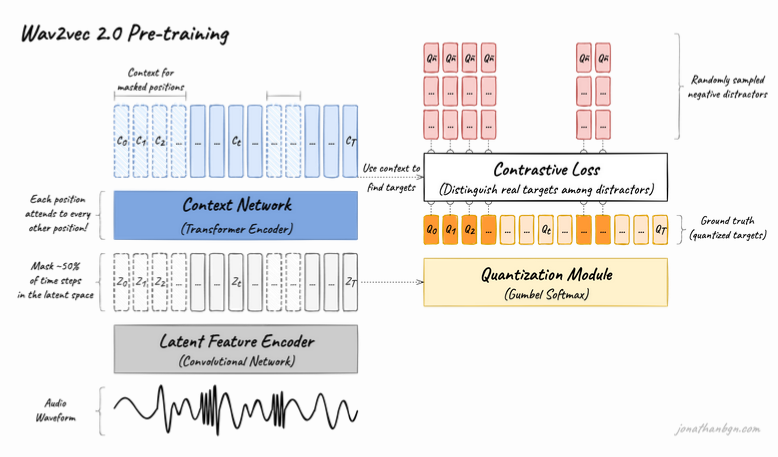
\includegraphics[width=0.8\textwidth]{wav2vec2-architecture.png}
    \caption{Arhitectura modelului \textit{wav2vec 2.0} \protect\footnotemark[1]}
    \label{fig:wav2vec2-architecture}
\end{figure}

\subsubsection{Latent Feature Encoder}
\vspace{3em}
Componenta Latent Feature Encoder este o rețea convoluțională care primește ca 
intrare un semnal audio și aplică o serie de operații de convoluție, normalizare
și activări GELU pentru a extrage caracteristici latente din semnalul audio.
\ref{fig:latent-feature-encoder}

\vspace{3em}

\begin{figure}[h]
    \centering
    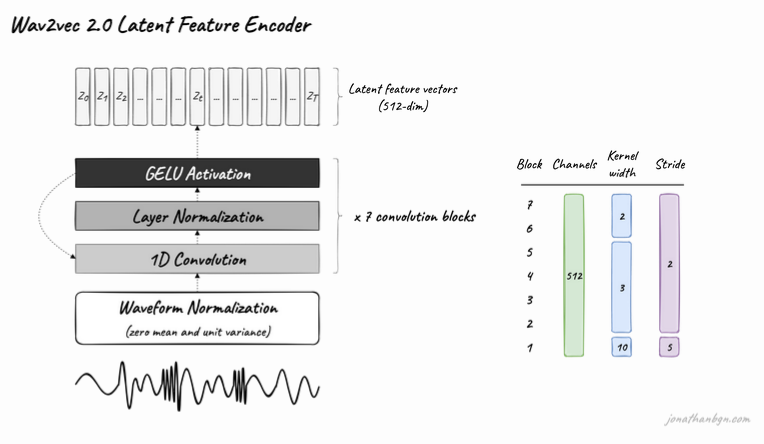
\includegraphics[width=0.8\textwidth]{wav2vec2-feature-encoder.png}
    \caption{Arhitectura componentei Latent Feature Encoder \protect\footnotemark[1]}
    \label{fig:latent-feature-encoder}
\end{figure}


\vspace{3em}

\subsubsection{Context Network}
\vspace{1em}
Componenta Context Network este un encoder de tip Transformer care primește ca
intrare caracteristicile latente extrase de componenta Latent Feature Encoder și
le procesează pentru a obține o reprezentare contextuală a semnalului audio. Aducând
aminte de arhitectura modelului anterior \textit{wav2vec} \cite{wav2vec}, care folosea
tot o rețea convoluțională la acest pas, ar părea că se aseamană cu componenta anterioară.
Diferența constă în faptul că Latent Feature Encoder urmărește să reducă dimensiunea 
semnalului audio, în timp ce Context Network urmărește să înțeleagă un context mai larg
al semnalului audio. \ref{fig:wav2vec2-context-network}

\begin{figure}[h]
    \centering
    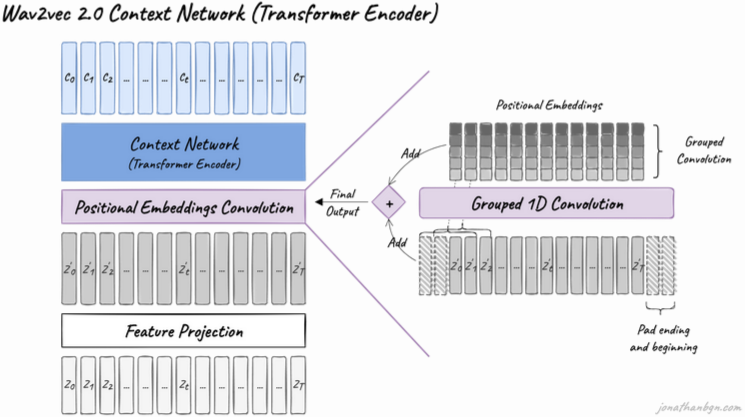
\includegraphics[width=0.8\textwidth]{wav2vec2-context-network.png}
    \caption{Arhitectura componentei Context Network \protect\footnotemark[1]}
    \label{fig:wav2vec2-context-network}
\end{figure}

\vspace{3em}

\subsubsection{Quantization Module} 
Deoarece modelul \textit{wav2vec 2.0} folosește pentru partea de Context Network un encoder de tip
Transformer, ne confruntăm cu problema structurii continue a semnalului audio. Limbajul scris poate
fi discretizat într-un set finit de simboluri, în timp ce semnalul audio nu permite în mod direct
acest lucru. Astfel, modelul \textit{wav2vec 2.0} folosește un modul de cuantizare care învață automat
unități de vorbire din semnalul audio. Intuitiv, se încearcă găsirea unor sunete fonetice 
finite și reprezentative pentru ieșirile din Latent Feature Encoder. De asemenea, se aplică 
funcția Gumbel Softmax \cite{gumbel-softmax}, funcție diferențiabilă care permite antrenarea modelului
prin backpropagation. \ref{fig:wav2vec2-quantization-module}

\begin{figure}[h]
    \centering
    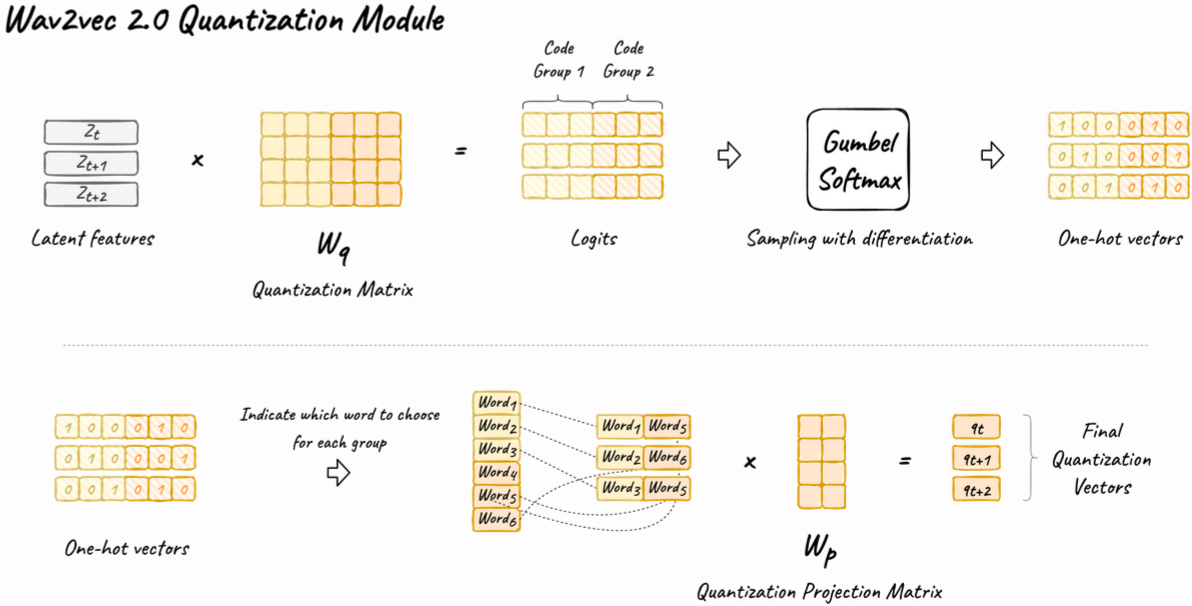
\includegraphics[width=0.8\textwidth]{wav2vec2-quantization-module.png}
    \caption{Arhitectura componentei Quantization Module \protect\footnotemark[1]}
    \label{fig:wav2vec2-quantization-module}
\end{figure}

\subsubsection{Contrastive Loss}
Pentru antrenarea modelului folosește o mască care ascunde ~50\% din vectorii proiectați din spațiul
latent înainte să fie trecuți prin Context Network. Acest lucru forțează modelul să învețe
reprezentări între vectorii proiectați și vectorii ascunși. Pentru fiecare poziție mascată, se
aleg uniform aleator 100 de exemple negative de la alte poziții și se compară similaritatea cosinus
între vectorul proiectat și vectorii aleși. Astfel, funcția de pierdere contrastivă încurajează
similaritatea cu exemplele true positive și penalizează similaritatea cu exemplele false positive.

\begin{figure}[h]
    \centering 
    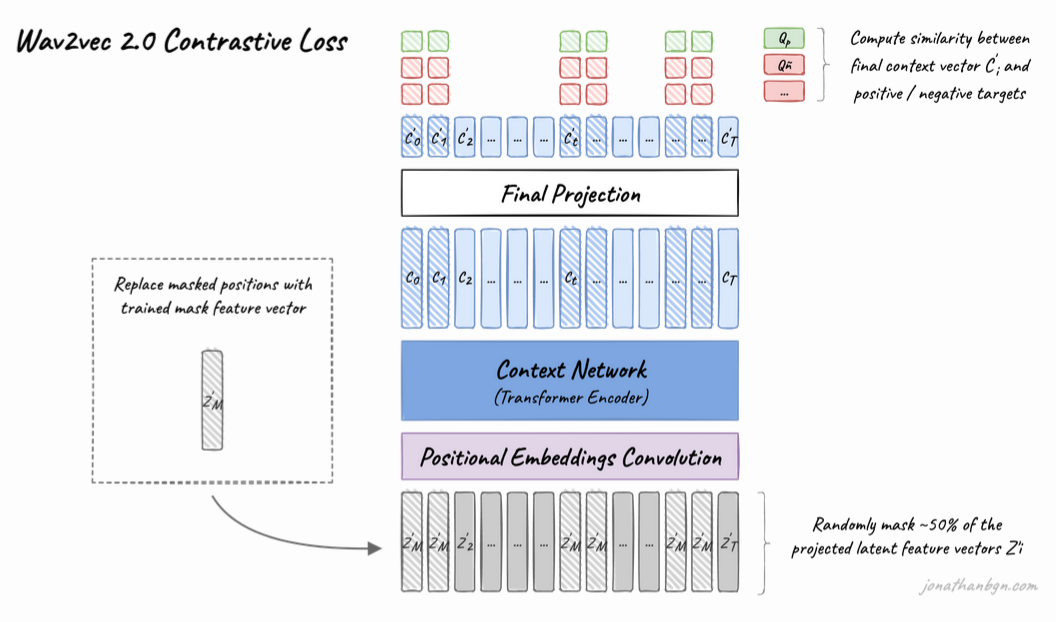
\includegraphics[width=0.8\textwidth]{wav2vec2-contrastive-loss.png}
    \caption{Arhitectura componentei Contrastive Loss \protect\footnotemark[1]}
    \label{fig:wav2vec2-contrastive-loss}
\end{figure}

\footnotetext[1]{Imaginile au fost preluate de pe site-ul lui Jonathan Bgn, ``Illustrated Wav2Vec 2.0'', disponibil la: \url{https://jonathanbgn.com/2021/09/30/illustrated-wav2vec-2.html}.}

\subsection{Setul de date}
Modelul oficial a fost preantrenat pe setul de date \textit{LibriSpeech}, iar eu am continuat
antrenarea pe seturile de date \textit{Mini LibriSpeech} și \textit{Common Voice Delta Segment 16.1}.

\subsubsection{Mini-LibriSpeech}
\textit{Mini LibriSpeech} este un subset al setului de date \textit{LibriSpeech} care conține 
aproximativ 2 ore de înregistrări audio la o frecvență de eșantionare de 16 kHz. În medie,
fiecare înregistrare are o durată de 6.72 secunde, cel mai lung audio având o durată de 31.5 secunde.

\subsubsection{Common Voice Delta Segment 16.1}
\textit{Common Voice Delta Segment 16.1} este un subset al setului de date \textit{Common Voice}
care conține aproximativ 2 ore de înregistrări audio la o frecvență de eșantionare de 48 kHz.
A fost nevoie să reduc frecvența de eșantionare la 16 kHz pentru a putea folosi aceste date la
antrenarea modelului. În medie, fiecare înregistrare are o durată de 5.63 secunde, cel mai lung
audio având o durată de 10.47 secunde.

\begin{figure}[h]
    \centering
    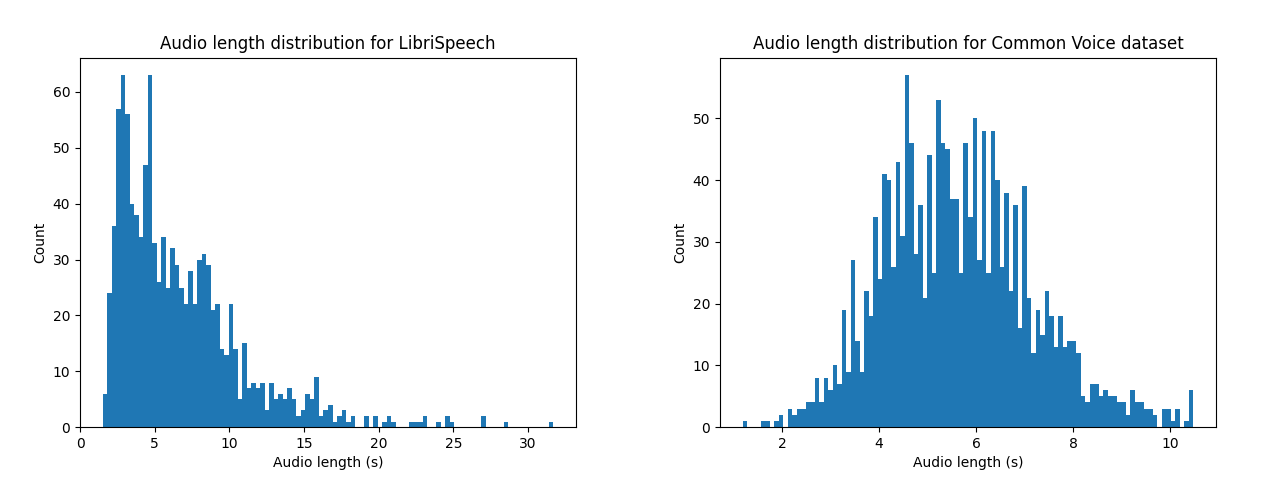
\includegraphics[width=0.8\textwidth]{length_distribution.png}
    \caption{Distribuția duratelor secvențelor audio din seturile de date \textit{Mini LibriSpeech} și \textit{Common Voice Delta Segment 16.1}}
    \label{fig:length-distribution}
\end{figure}

\subsubsection{Concluzie}
Menționez aceste detalii deoarece pentru generarea subtitrărilor vom avea nevoie de audio-uri
mult mai lungi decât cele folosite pentru antrenare care nu ar încăpea în memorie. Astfel, va trebui
să folosim o tehnică de segmentare a secvențelor audio în bucăți mai mici pentru a putea fi procesate.
Mai multe detalii despre această tehnică vor fi prezentate în secțiunea \textit{Subtitrări}.

\subsection{Antrenarea modelului}
Pentru antrenarea modelului am folosit limbajul de programare Python și biblioteca Hugging Face
care pune la dispoziție o serie de pachete precum \textit{transformers} și \textit{datasets}.
\par
Hiperparametrii folosiți pentru fine-tuning-ul modelului sunt:
\begin{itemize}
    \item \textbf{Learning rate} - pentru a controla cât de mult se modifică gradienții în timpul
    antrenării 
    \item \textbf{Weight decay} - pentru a controla cât de mult se penalizează valorile mari ale
    parametrilor 
    \item \textbf{Warmup steps} - pentru a controla cât de mult se modifică learning rate-ul în
    primele pași ai antrenării
    \item \textbf{Batch size} - câte exemple se procesează în același timp
\end{itemize}

\vspace{0.5em}

\begin{table}[h]
    \centering
    \label{tab:wav2vec2-hyperparameters}
    \begin{tabular}{ll}
    \hline
    \textbf{Hiperparametru} & \textbf{Valoare} \\ \hline
    Rata de învățare (\textit{learning rate}) & $1 \times 10^{-4}$ \\
    Descreșterea greutății (\textit{weight decay}) & 0.005 \\
    Pași de încălzire (\textit{warmup steps}) & 1000 \\
    Dimensiunea lotului (\textit{batch size}) & 4 \\ \hline
    \end{tabular}
    \caption{Hiperparametrii folosiți pentru fine-tuning-ul modelului \textit{wav2vec2}}
\end{table}

\par
Am antrenat modelul pe seturile de date \textit{Mini LibriSpeech} și \textit{Common Voice Delta Segment 16.1}
pe o placă grafică NVIDIA Tesla V100 pusă la dispoziție de Google Colab. Am făcut un checkpoint la fiecare
500 de pași pentru a putea monitoriza evoluția modelului. Rezultatele checkpoint-urilor pentru modelul
\textit{facebook/wav2vec2-base} sunt prezentate în cele două tabele de mai jos.


% \begin{figure}[h]
%     \centering
%     \begin{minipage}{.5\textwidth}
%         \centering
%         \captionsetup{justification=centering} 
%         \captionof{table}{Mini LibriSpeech}
%         \label{tab:model-checkpoints1}
%         \begin{tabular}{cccc}
%         \toprule
%         \textbf{Step} & \textbf{Train loss} & \textbf{Val loss} & \textbf{wer(\%)} \\
%         \midrule
%         500  & 3.840 & 3.099 & 1.000 \\
%         1000 & 1.202 & 0.586 & 0.361 \\
%         1500 & 0.360 & 0.352 & 0.265 \\
%         2000 & 0.231 & 0.333 & 0.222 \\
%         2500 & 0.163 & 0.357 & 0.230 \\
%         3000 & 0.136 & 0.331 & 0.199 \\
%         3500 & 0.114 & 0.369 & 0.205 \\
%         4000 & 0.104 & 0.348 & 0.203 \\
%         4500 & 0.094 & 0.335 & 0.177 \\
%         5000 & 0.083 & 0.284 & 0.165 \\
%         5500 & 0.078 & 0.332 & 0.165 \\
%         6000 & 0.072 & 0.356 & 0.174 \\
%         6500 & 0.069 & 0.393 & 0.165 \\
%         7000 & 0.066 & 0.380 & 0.181 \\
%         \bottomrule
%         \end{tabular}
%     \end{minipage}%
%     \begin{minipage}{.5\textwidth}
%         \centering
%         \captionof{table}{Common Voice Delta 16.1}
%         \label{tab:model-checkpoints2}
%         \begin{tabular}{cccc}
%         \toprule
%         \textbf{Step} & \textbf{Train loss} & \textbf{Val loss} & \textbf{wer(\%)} \\
%         \midrule
%         500  & 3.919 & 3.236 & 1.000 \\
%         1000 & 1.287 & 0.570 & 0.398 \\
%         1500 & 0.368 & 0.400 & 0.261 \\
%         2000 & 0.226 & 0.371 & 0.252 \\
%         2500 & 0.166 & 0.402 & 0.239 \\
%         3000 & 0.136 & 0.475 & 0.233 \\
%         3500 & 0.116 & 0.445 & 0.201 \\
%         4000 & 0.097 & 0.448 & 0.196 \\
%         4500 & 0.096 & 0.404 & 0.190 \\
%         5000 & 0.079 & 0.459 & 0.182 \\
%         5500 & 0.080 & 0.400 & 0.182 \\
%         6000 & 0.069 & 0.445 & 0.182 \\
%         6500 & 0.073 & 0.421 & 0.179 \\
%         7000 & 0.064 & 0.440 & 0.182 \\
%         \bottomrule
%         \end{tabular}
%     \end{minipage}
% \end{figure}
    
\begin{figure}[h]
    \centering
    \begin{minipage}{.5\textwidth}
        \centering
        \captionsetup{justification=centering} 
        \captionof{table}{Mini LibriSpeech}
        \label{tab:model-checkpoints1}
        \begin{tabular}{ccc}
        \toprule
        \textbf{Step} & \textbf{Train loss} & \textbf{Val loss} \\
        \midrule
        500  & 3.840 & 3.099 \\
        1000 & 1.202 & 0.586 \\
        1500 & 0.360 & 0.352 \\
        2000 & 0.231 & 0.333 \\
        2500 & 0.163 & 0.357 \\
        3000 & 0.136 & 0.331 \\
        3500 & 0.114 & 0.369 \\
        4000 & 0.104 & 0.348 \\
        4500 & 0.094 & 0.335 \\
        5000 & 0.083 & 0.284 \\
        5500 & 0.078 & 0.332 \\
        6000 & 0.072 & 0.356 \\
        6500 & 0.069 & 0.393 \\
        7000 & 0.066 & 0.380 \\
        \bottomrule
        \end{tabular}
    \end{minipage}%
    \begin{minipage}{.5\textwidth}
        \centering
        \captionof{table}{Common Voice Delta 16.1}
        \label{tab:model-checkpoints2}
        \begin{tabular}{ccc}
        \toprule
        \textbf{Step} & \textbf{Train loss} & \textbf{Val loss} \\
        \midrule
        500  & 3.919 & 3.236 \\
        1000 & 1.287 & 0.570 \\
        1500 & 0.368 & 0.400 \\
        2000 & 0.226 & 0.371 \\
        2500 & 0.166 & 0.402 \\
        3000 & 0.136 & 0.475 \\
        3500 & 0.116 & 0.445 \\
        4000 & 0.097 & 0.448 \\
        4500 & 0.096 & 0.404 \\
        5000 & 0.079 & 0.459 \\
        5500 & 0.080 & 0.400 \\
        6000 & 0.069 & 0.445 \\
        6500 & 0.073 & 0.421 \\
        7000 & 0.064 & 0.440 \\
        \bottomrule
        \end{tabular}
    \end{minipage}
\end{figure}

\subsubsection{Note}
Se observă că modelul a început să învețe destul de repede, scăzând pierderea de antrenare
de la 3.840 la 0.066, respectiv de la 3.919 la 0.064 în doar 7000 de pași. Urmărind graficul,
se observă fenomenul de \textit{overfitting} care apare în jurul pașilor 5000-6000, motiv
pentru care am ales să opresc antrenarea la 7000 de pași și sa folosesc checkpoint-ul de
la pasul 5000, respectiv 5500.


% CITESTE INAINTE SA CONTINUI SA SCRII
% wer pare ca nu arata valorile corecte la antrenare
% ai testat in scriptul test.py modelul normal si modelul cu language model
% si ai obtinut valori corecte pentru wer

% - explica cum merge n-gram language model
% - arata imbunatatirea (ruleaza script ul test.py)
% - eventual fa discutie si despre fix spelling

\subsection{Îmbunătățire cu n-gram language model}
Pentru a îmbunătăți recunoașterea vorbirii, am folosit un n-gram language model care 
mărește performanța modelului de la \textbf{wer 4.2\%}  la \textbf{wer 2.9\%}, aducând
o îmbunătățire de \textbf{1.3\%}.

\subsubsection{N-gram Language Model}
Un n-gram language model este un model statistic care estimează, în cazul nostru, probabilitatea
apariției unui caracter având în vedere cele n-1 caractere anterioare. Modelul se bazează pe
ipoteza Markov de ordinul n, conform căreia putem aproxima probabilitatea apariției unui caracter
folosind doar ultimele n caractere. Formula de mai jos ilustreaza această idee.

\begin{equation}
    P(w_1, w_2, \ldots, w_n) = \prod_{i=1}^{m} P(w_i | w_{1}, w_{2}, \ldots, w_{i-1}) \approx \prod_{i=1}^{m} P(w_i | w_{i-(n-1)}, \ldots, w_{i-1})
\end{equation}
\vspace{1em}

\par
Am folosit un context de 5 caractere și am antrenat modelul pe
setul de date \textit{Helsinki-NLP/europarl} \cite{tiedemann-2012-parallel} deoarece conține și
texte în limba engleză și putem avea certitudinea că textele sunt corecte din punct de vedere
gramatical. Cu ajutorul librăriei \textit{KenLM} \cite{heafield-2011-kenlm}, am antrenat modelul
de n-grame și apoi am creat un procesor specific Hugging Face pentru modelele \textit{wav2vec 2.0}.

\par
În mod normal, modelul \textit{wav2vec 2.0} ia argumentul maxim din distribuția de probabilitate
pentru a prezice caracterul următor. În schimb, cu ajutorul n-gram language model, aceste
probabilități sunt alterate pentru a se apropia de limbajul natural. 

\subsubsection{Îmbunătățire cu Transformer Language Model}
\vspace{1em}
Având în vedere performanța arhitecturii Transformer în învățarea secvențelor, o altă abordare
ar fi utilizarea unui model de limbaj bazat pe Transformer. Paper-ul original \cite{wav2vec2}
menționează în Appendix-ul C că un model de limbaj bazat pe Transformer este într-adevăr mai
bun decât un model de limbaj bazat pe n-grame, dar durata antrenării și a inferenței este
mult mai mare. 
\par 
Tabelul de mai jos a fost extras din paper-ul original și prezintă rezultatele obținute. \ref{fig:boost-results}

\begin{figure}[h!]
    \centering
    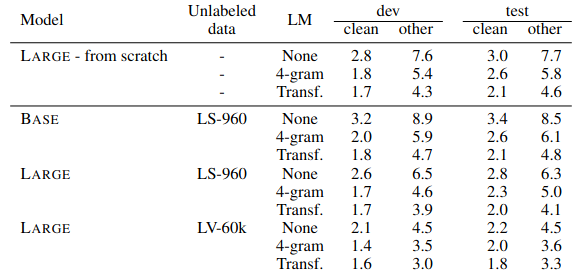
\includegraphics[width=0.8\textwidth]{boost-results.png}
    \caption{Rezultatele obținute cu un model simplu, un model de limbaj bazat pe n-grame și un model de limbaj bazat pe Transformer}
    \label{fig:boost-results}
\end{figure}


\section{Clasificarea videoclipurilor}
Videoclip-urile încărcate pe platform vin însoțite de metadate precum: titlu, descriere și, folosind
modelul prezentat anterior, subtitrări. Pentru o experiță mai personalizată, am ales să clasific
videoclipurile în funcție de subiectul abordat în topicuri precum: politics, sport, entertainment
tehnologie și afaceri. Am folosit un modelul de clasificare \textit{BERT}, Bidirectional Encoder Representations
from \textit{Transformers}, dezvoltat de \textit{Google} \cite{devlin2019bert} pe care l-am antrenat pe setul de date
\textit{BBC News} \cite{greene06icml}.

\subsection{Arhitectura modelului}
Modelul \textit{BERT} este un model de învățare profundă care are la bază partea de encoder a unui \textit{Transformer} \cite{vaswani2023attention},
scopul lui fiind de a înțelege contextul cuvintelor într-o propoziție. Modelul \textit{BERT} vine în două
variante: \textit{BERT-base} și \textit{BERT-large}, cele două diferă prin numărul de blocuri de encoder (12 și 24),
numărul de neuroni din stratul fully-connected (768 și 1024) și numărul de attention heads (12 și 16), dar 
conceptual sunt la fel. 

\par
Spre deosebire de arhitectura standard a unui \textit{Transformer}, \textit{BERT} adaugă un token
special la începutul fiecărei propoziții, \textit{[CLS]}, folosit pentru clasificare. Intuitiv,
acest token va reține informații despre întreaga propoziție și va putea fi folosit pentru rețeaua
de clasificare care va determina topicul propoziției. \ref{fig:bert-architecture}

\begin{figure}[h]
    \centering
    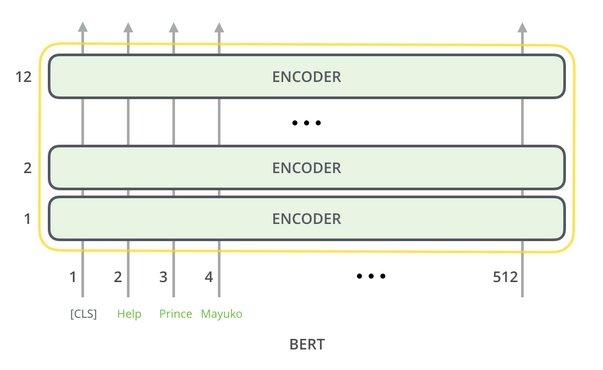
\includegraphics[width=0.8\textwidth]{bert-architecture.png}
    \caption{Arhitectura modelului \textit{BERT} \protect\footnotemark[2]}
    \label{fig:bert-architecture}
\end{figure}
\vspace{1em}

\par
Ieșirile modelului \textit{BERT} au dimensiunea 768, iar pentru partea de clasificare sunt trecute
prin un strat fully-connected cu 5 neuroni, câte unul pentru fiecare clasă. Cu ajutorul funcției
\textit{softmax}, se obține o distribuție de probabilitate peste cele 5 clase, iar clasa cu cea mai
mare probabilitate este cea aleasă.

\footnotetext[2]{Imaginea a fost preluată de pe site-ul lui Jay Alammar, ``The Illustrated BERT, ELMo, and co. (How NLP Cracked Transfer Learning)'', disponibil la: \url{https://jalammar.github.io/illustrated-bert/}.}

\vspace{1em}

\subsection{Setul de date}
\vspace{1em}
Pentru antrenarea modelului am folosit setul de date \textit{BBC News} care conține 2225 de articole 
între anii 2004-2005. Setul de date este împărțit în 5 clase: politics, sport, entertainment, technology
și business. Mai jos am prezentat distribuția datelor din setul de date din punct de vedere al exemplelor
pe clasă și al lungimii medii a articolelor. \ref{fig:bbc-stats}

\vspace{1em}

\begin{figure}[h]
    \centering
    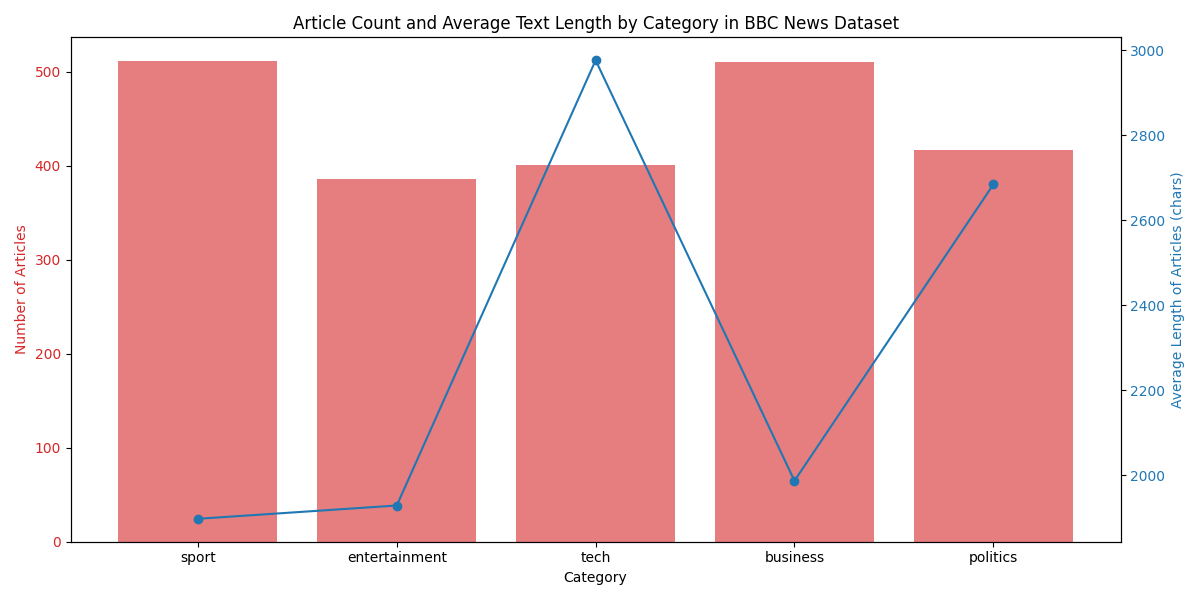
\includegraphics[width=0.8\textwidth]{bbc_stats.png}
    \caption{Distribuția claselor din setul de date \textit{BBC News}}
    \label{fig:bbc-stats}
\end{figure}


\subsection{Antrenarea modelului}
\vspace{1em}
Antrenarea modelului a fost făcută folosind limbajul de programare Python, biblioteca PyTorch. \cite{paszke2019pytorch}
și plecând de la modelul preantrenat \textit{bert-base-uncased} pus la dispoziție de Hugging Face.
Codul a fost structurat în: 
\vspace{1em}

\begin{itemize}
    \item \textbf{dataset.py} - creează un Dataset specific PyTorch pentru setul de date \textit{BBC News},
    implementând metodele \textit{\_\_len\_\_} și \textit{\_\_getitem\_\_}; metoda \textit{\_\_getitem\_\_}
    aplică tokenizer-ul pe text cu lungimea maximă de 512 token-uri și returnează un tuplu de input\_ids,
    attention\_mask și label
    \item \textbf{model.py} - definește arhitectura modelului \textit{BERT} și a rețelei de clasificare:
    inițializează modelul preantrenat \textit{bert-base-uncased}, extrage token-ul special \textit{[CLS]}
    și adaugă un strat liniar cu 5 neuroni pentru clasificare
    \item \textbf{trainer.py} - antrenează modelul pe setul de date \textit{BBC News} folosind hiperparametrii
    din primiți ca parametru în linia de comandă și salvează modelul de fiecare dată când obține o
    acuratețe mai bună pe setul de validare
\end{itemize}

\vspace{1em}

\par
În figurile de mai jos \ref{fig:loss_graphs} sunt ilustrate pierderile de antrenare și de evaluare pentru modelul \textit{BERT}
folosind ca rată de învățare $1 \times 10^{-4}$ și $1 \times 10^{-5}$. Se observă fenomenul de \textit{overfitting}
pentru rata de învățare $1 \times 10^{-4}$, motiv pentru care am ales să experimentez cu valori mai mici.

\begin{figure}[ht]
    \centering
    \begin{subfigure}[b]{0.45\textwidth}
        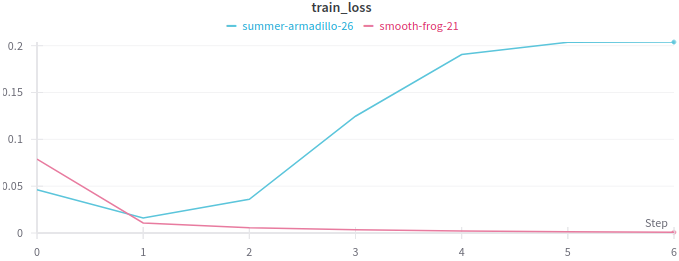
\includegraphics[width=\textwidth]{train_loss_1.png}
        \caption{Training Loss}
        \label{fig:train_loss}
    \end{subfigure}
    \hfill % Asigură spațierea dintre subfiguri
    \begin{subfigure}[b]{0.45\textwidth}
        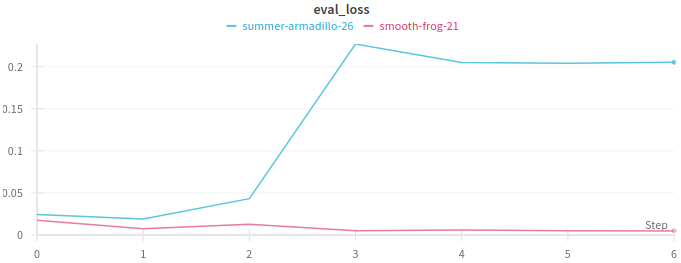
\includegraphics[width=\textwidth]{eval_loss_1.png}
        \caption{Evaluation Loss}
        \label{fig:eval_loss}
    \end{subfigure}
    \caption{Training and Evaluation Loss Graphs}
    \label{fig:loss_graphs}
\end{figure}
\vspace{1em}

\par
Am încercat mai multe experimente plecând de la aceeași hiperparametri, cu rata de învățare $1 \times 10^{-5}$,
pentru a vedea cum se comportă modelul la diferite inițializări ale ponderilor. În figura \ref{fig:eval_acc}
sunt ilustrate valorile obținute pentru acuratețea modelului pe setul de validare.


\begin{figure}[h]
    \centering
    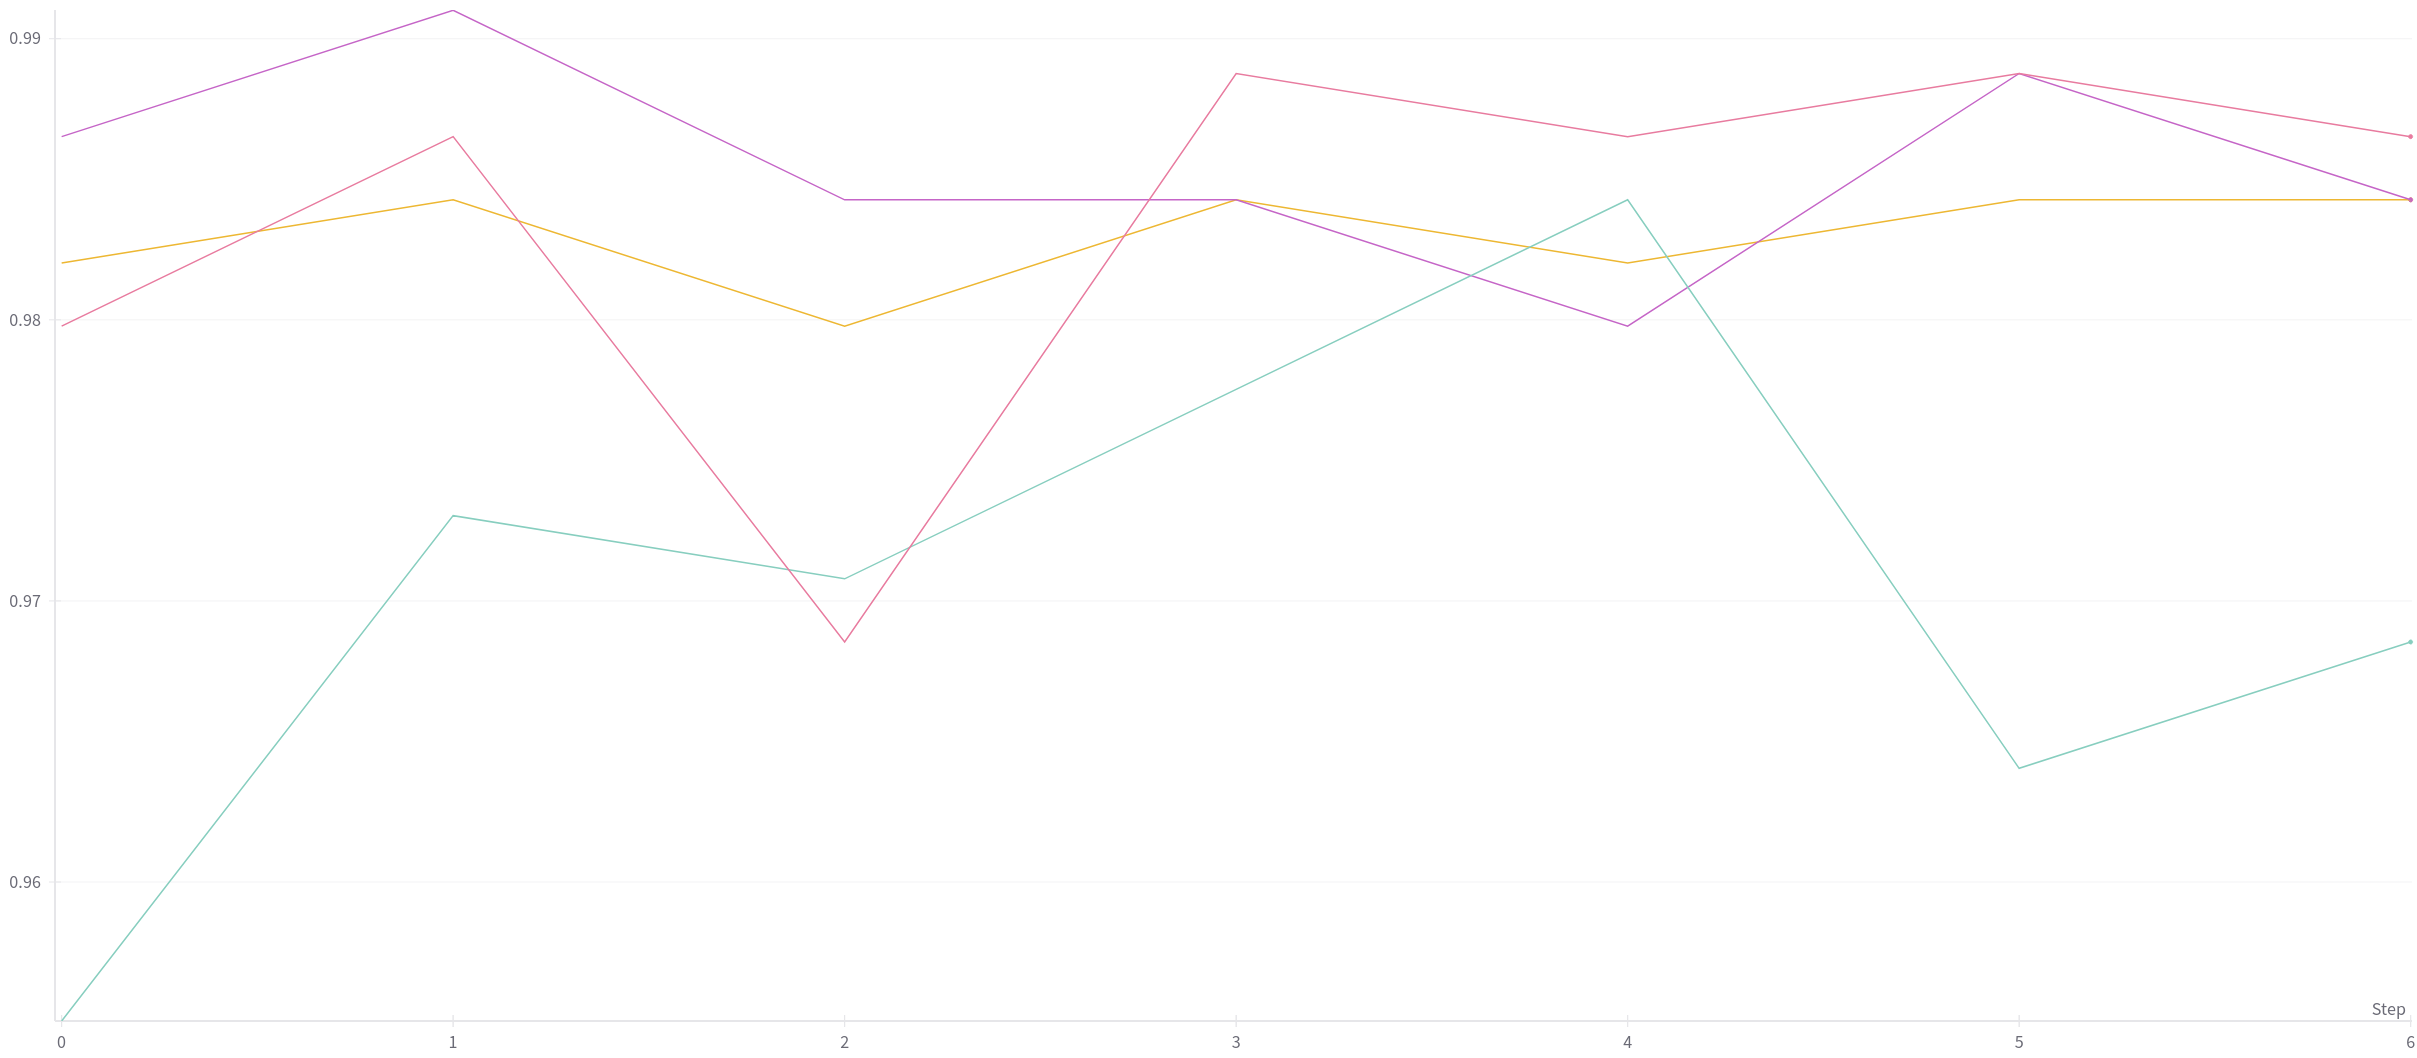
\includegraphics[width=0.8\textwidth]{eval_acc.png}
    \caption{Evaluation Accuracy Graph}
    \label{fig:eval_acc}
\end{figure}

\subsubsection{Hiperparametrii}
Pentru modelul final pe care l-am folosit pentru clasificarea videoclipurilor am ales următorii hiperparametrii:

% \begin{table}[h]
%     \centering
%     \label{tab:wav2vec2-hyperparameters}
%     \begin{tabular}{ll}
%     \hline
%     \textbf{Hiperparametru} & \textbf{Valoare} \\ \hline
%     Rata de învățare (\textit{learning rate}) & $1 \times 10^{-4}$ \\
%     Descreșterea greutății (\textit{weight decay}) & 0.005 \\
%     Pași de încălzire (\textit{warmup steps}) & 1000 \\
%     Dimensiunea lotului (\textit{batch size}) & 4 \\ \hline
%     \end{tabular}
%     \caption{Hiperparametrii folosiți pentru fine-tuning-ul modelului \textit{wav2vec2}}
% \end{table}

\begin{table}[ht]
    \centering
    \begin{tabular}{@{}ll@{}}
        \toprule
        \textbf{Hiperparametru}   & \textbf{Valoare}         \\
        \midrule
        Rata de învățare \textit{(learning rate)}             & 0.00001                  \\
        Dimensiunea lotului \textit{(batch size)}             & 8                        \\
        Optimizator \textit{(optimizer)}                      & Adam                     \\
        Funcția de pierdere \textit{(loss function)}          & CrossEntropyLoss         \\
        \bottomrule
    \end{tabular}
    \caption{Hiperparametrii modelului \textit{BERT}}
    \label{tab:bert-hyperparameters}
\end{table}


\section{Concluzie}
Cele două modele prezentate anterior, \textit{wav2vec 2.0} și \textit{BERT}, au fost încărcate
pe platforma Huggingface și sunt disponibile în pachetul \textit{transformers}.

\subsubsection{wav2vec 2.0}
Utilizarea modelului de recunoaștere a vorbirii necesită folosirea modulului \textit{Wav2Vec2ForCTC}
și a modulului \textit{Wav2Vec2Processor} sau \textit{Wav2Vec2ProcessorWithLM} pentru a folosi varianta
îmbunătățită cu n-grame. Codul de mai jos ilustrează cum se pot folosi modelele prezentate anterior.

\begin{lstlisting}[language=Python]
    from transformers import Wav2Vec2ForCTC, Wav2Vec2Processor, Wav2Vec2ProcessorWithLM
    
    asr_repos = {
        "minilibrispeech": "3funnn/wav2vec2-base-minilibrispeech",
        "common-voice": "3funnn/wav2vec2-base-common-voice",
    }
    lm_boosted_repos = {
        "minilibrispeech": "3funnn/wav2vec2-base-minilibrispeech-lm",
        "common-voice": "3funnn/wav2vec2-base-common-voice-lm",
    }
    
    repo_name = "minilibrispeech"
    boost_lm = True
    model = Wav2Vec2ForCTC.from_pretrained(asr_repos[repo_name])
    
    if boost_lm:
        processor = Wav2Vec2ProcessorWithLM.from_pretrained(lm_boosted_repos[repo_name])
    else:
        processor = Wav2Vec2Processor.from_pretrained(asr_repos[repo_name])
    \end{lstlisting}


\subsubsection{BERT}
Modelul de clasificare a videoclipurilor este disponibil în pachetul \textit{transformers} sub numele
\textit{3funnn/bert-topic-classification}. Modelul primește ca intrare un text care poate fi o 
concatenare a titlului și descrierii videoclipului și returnează o distribuție de probabilitate
pentru fiecare din cele 5 clase. Huggingface pune la dispoziție funcția \textit{pipeline} care
permite folosirea modelului într-un mod simplu. Codul de mai jos ilustreaza acest lucru.

\begin{lstlisting}[language=Python]
    from transformers import pipeline
    
    classifier = pipeline("text-classification", model="3funnn/bert-topic-classification")
    
    text = "This is a video about the latest technology in AI."
    result = classifier(text)
    print(result)
    # Output: {'label': 'tech', 'score': 0.897}
\end{lstlisting}
